%!tikz editor 1.0
\documentclass[beamer]{standalone}
\usepackage{tikz}
\usepackage{lmodern}

%!tikz preamble begin
\usepackage{tikz}
\usetikzlibrary{arrows,positioning,fit}
\usetikzlibrary{overlay-beamer-styles}

\xdefinecolor{color1}{rgb}{1.0, 0, 0}
\xdefinecolor{color2}{rgb}{0, 0.5, 1.0}

\tikzset{
    p1/.style={circle, draw, thick, minimum size=6mm, inner sep=0},
    p2/.style={rectangle, draw, thick, minimum size=5mm, inner sep=0},
    pre/.style = {<-, semithick, >=stealth', shorten <=1pt},
    post/.style= {->, semithick, >=stealth', shorten >=1pt},
  }
%!tikz preamble end

\begin{document}
\begin{standaloneframe}
%!tikz source begin
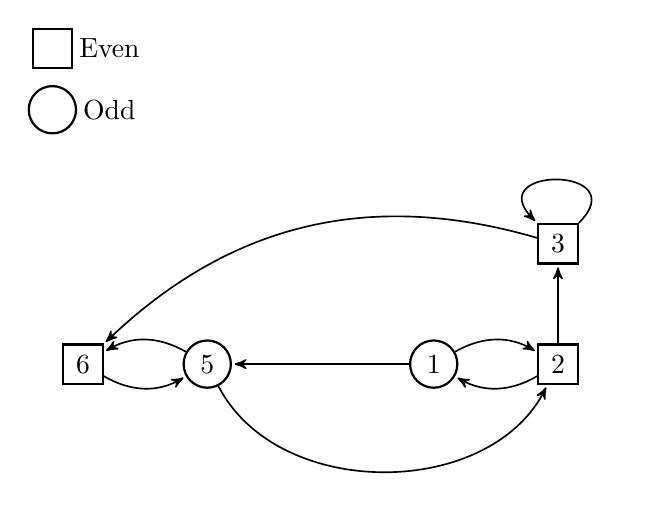
\begin{tikzpicture}[podd/.style=p1, peven/.style=p2]
      \node (origin) at (0,0) {};
      	\node (5) [podd, left=of origin] {5};
      	\node (6) [peven, left=of 5]  {6}
      		edge [pre,bend left] (5)
      		edge [post, bend right] (5);
      	\node (1) [podd, right=of origin]  {1}
  			edge [post] (5);
      	\node (2) [peven, right=of 1]  {2}
  			edge [post, bend left] (1)
  			edge [pre, bend right] (1)
  			edge [pre, bend left=63] (5);
      	\node (3) [peven, above=of 2] {3}
        	edge [post, loop, looseness=5] (3)
  		    edge [pre] (2)
            edge [post, bend right] (6);

  		\node (graph) [fit=(1) (2) (3) (6) (5)] {};
      \begin{scope}[inner sep=2pt, minimum size=1pt]
        \node (odd-sym) [podd, above=of graph.north west , label={right:Odd}] {};
    		\node [peven, above=2mm of odd-sym, label={right:Even}] {};
      \end{scope}
  \end{tikzpicture}
\end{standaloneframe}
%!tikz source end
\end{document}
